\subsection{File characterization}

After analyzing layers and images, we conducted a deeper analysis on the files that are stored in containers.% by compressing and upacking the layer 
Specifically, we characterize files in terms of size and type.   
%present file size distribution and clustering file types.
%In this section, we present our redundant file characterization on file repeat count 
Based on this characterization, we create three-level classification hierarchy as shown in Figure~\ref{fig:file-type-hierarchy}.
At the highest level, we created two categories: \textit{Common used file types and non-common used file types} based on the total file size and file count for each type. 
Totally, we got around 1,500 types after analyzing our whole dataset. 
We found that only 133 file types that take up more than 7 GB individually and occupy the most of capacity (98.4\%, with 166.8 TB) totally.
%'s total file sizes are greater than 5 GB, which take up to  
%files with 166.8 TB totally. 
We put these 133 file types into common used file type group and the remaining files into non-common used file types. Our further classification expands on the 98.4\% common used file types. 
%
%are common file types that consists of a largest number of redundant files with large storage space consumed, such as xxx and xxx. 
%Only xxxx\% files are non-common file types that only contains a small number of redundant files with less storage space, such as xxxx and xxxx. 

At the second level of the hierarchy, we clustered common used file types based on the \textit{major file format, usage, or platform} involved by each file type. We identified common used file types relevant to \textit{EOF (executable, object code, and libraries), source code, scripts, documents, archival, images, databases, and others}.

At the third level, we present the specific redundant file types which take a large percentage of redundant files or storage space.

\begin{figure*}
	\centering
	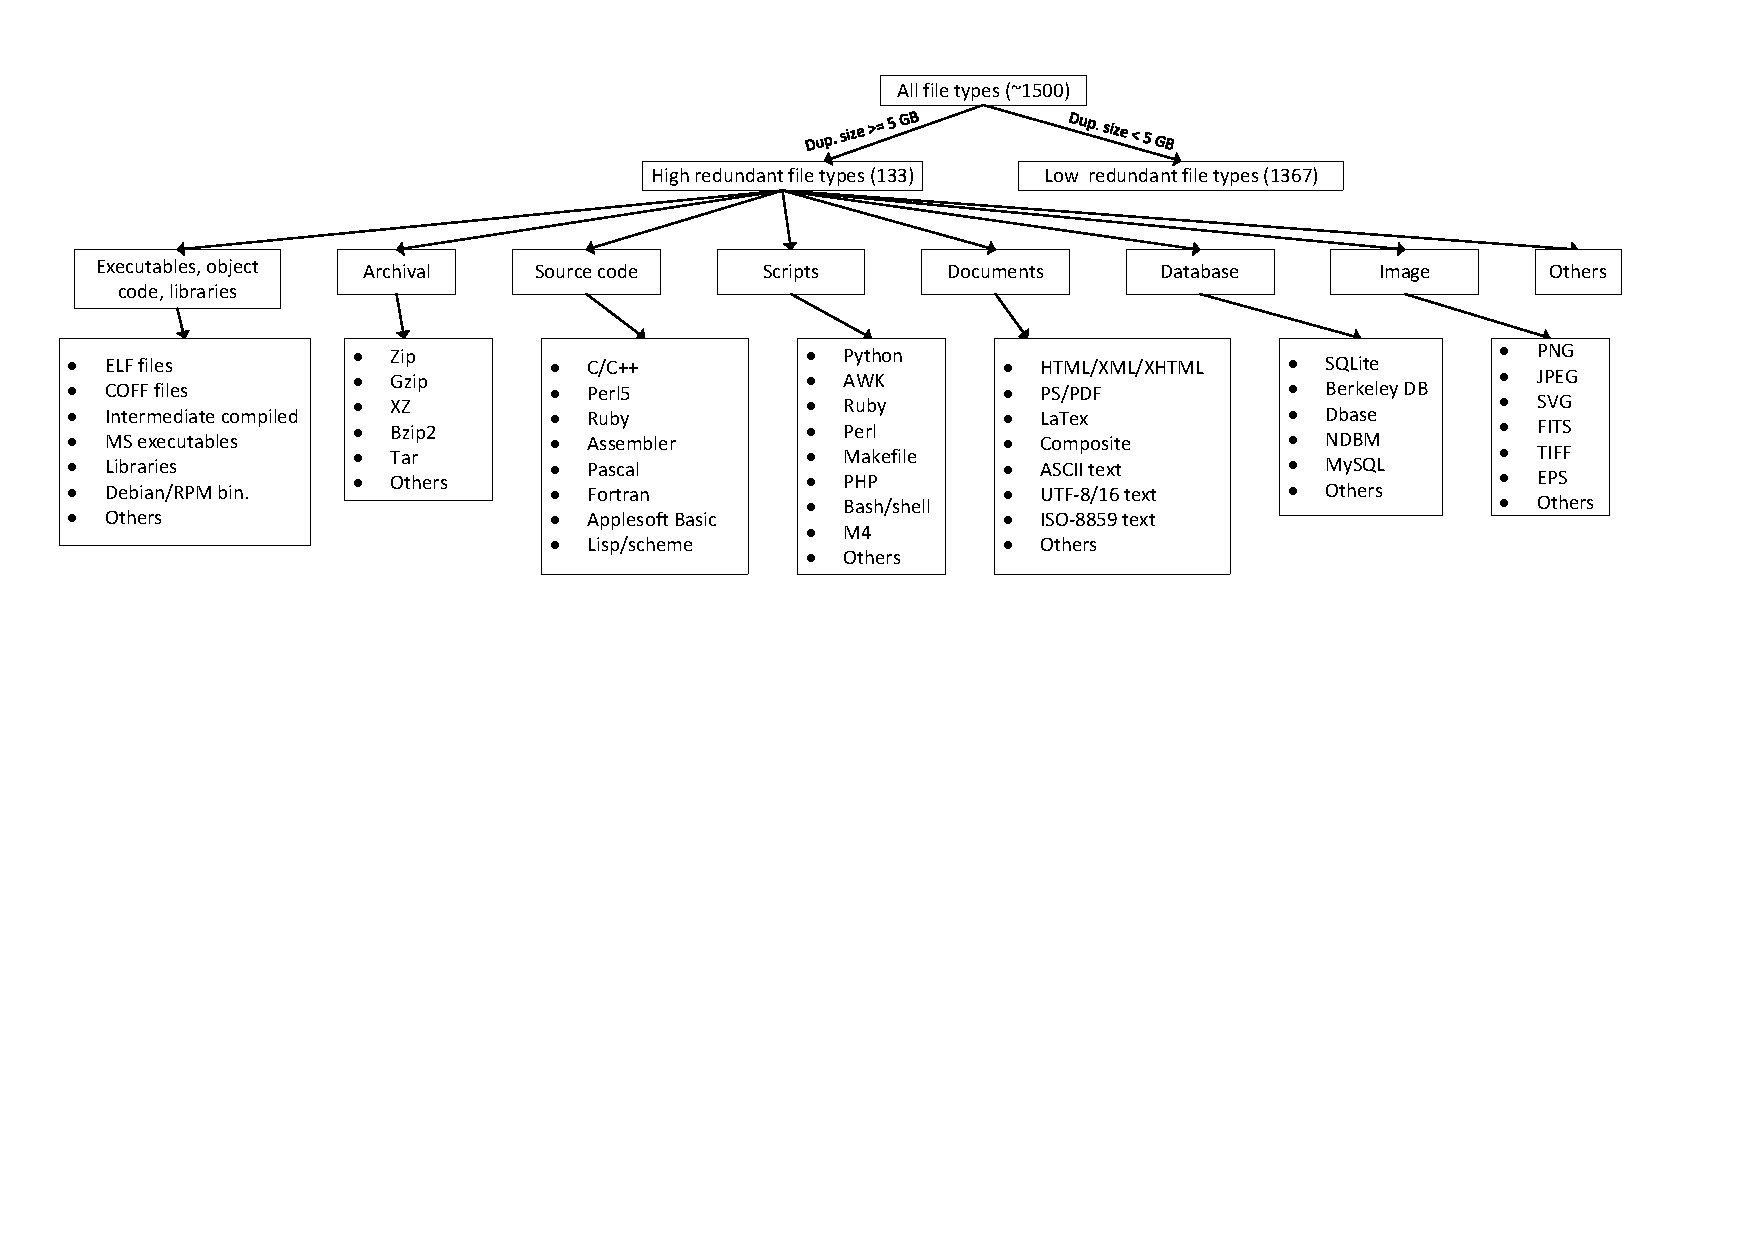
\includegraphics[width=1\textwidth]{graphs/graph-types-hierarchy}
	\caption{Taxonomy of file types.
	}
	\label{fig:file-type-hierarchy}
\end{figure*}

\paragraph{Common used file types}

\begin{figure}
	\centering
	\subfigure[File count (in \%) by file type group.]{\label{fig:type-total-cnt}
		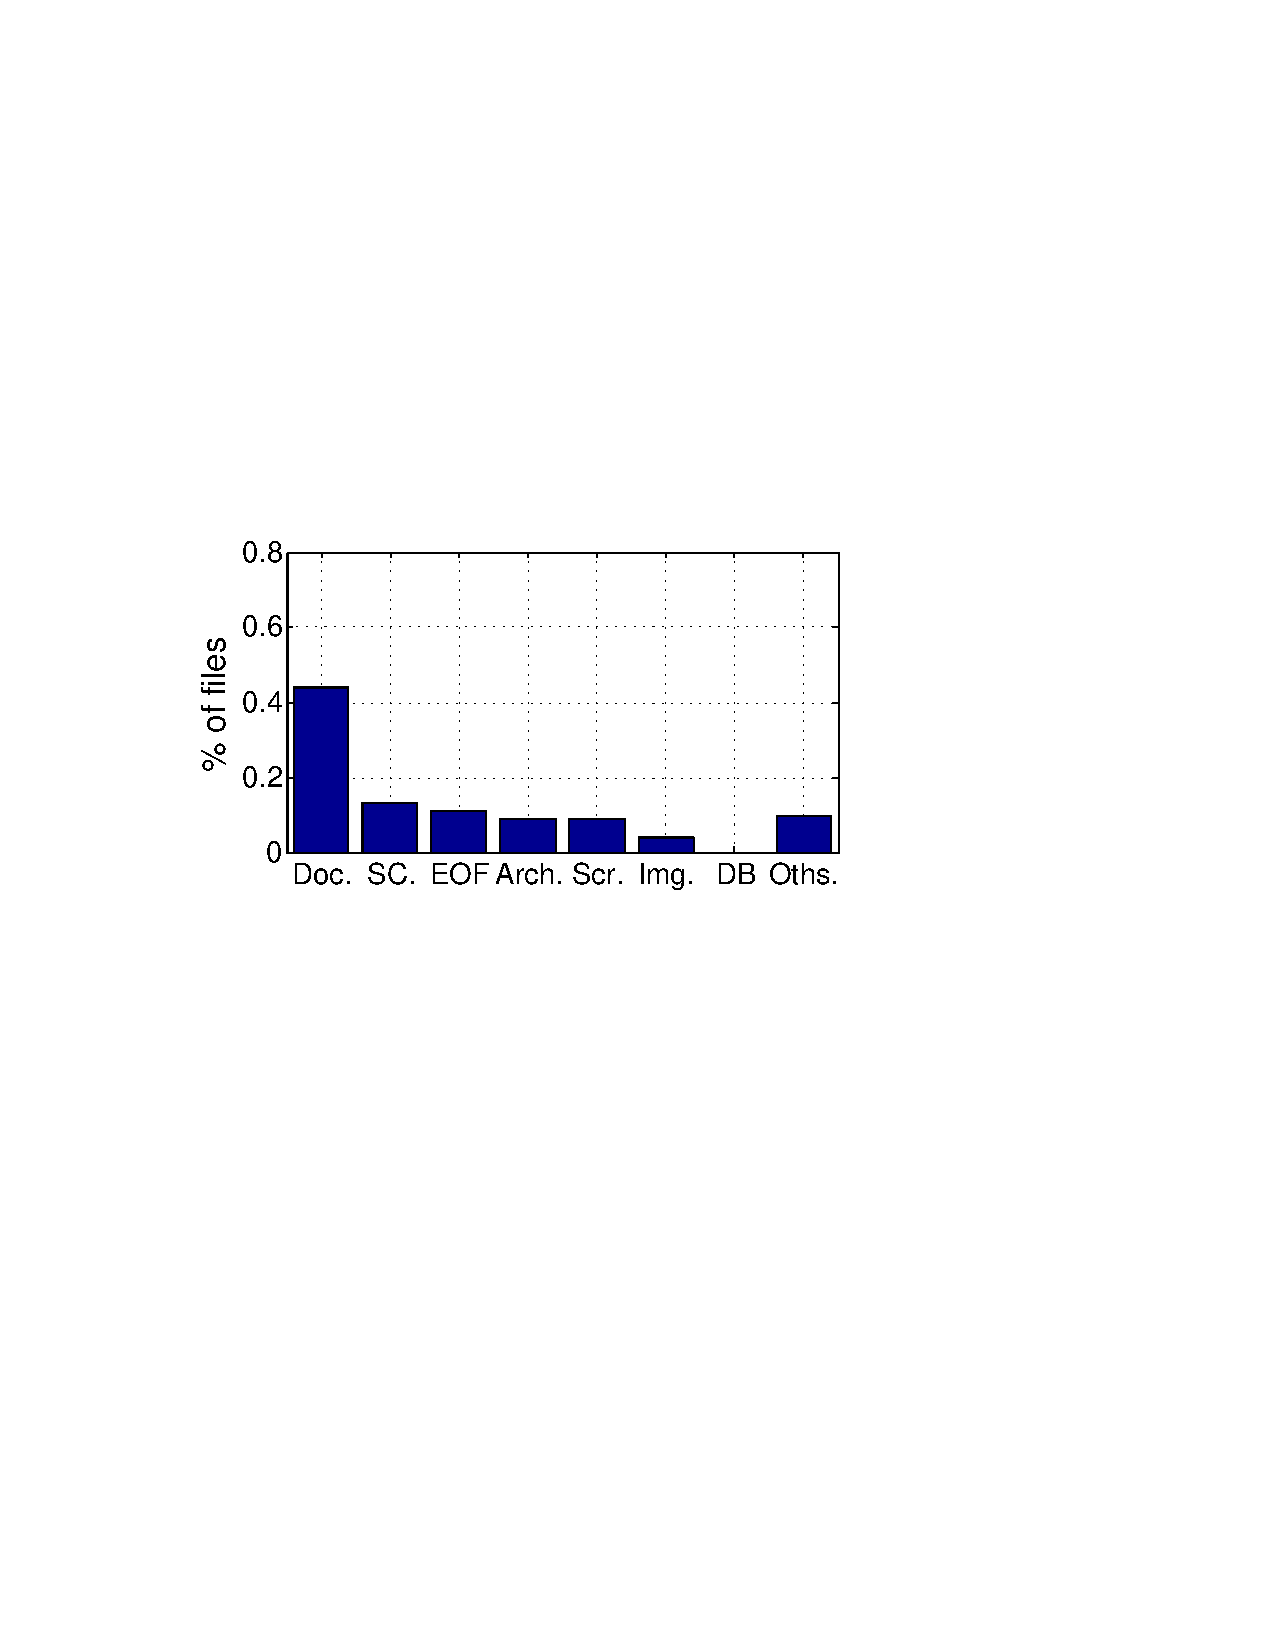
\includegraphics [width=0.225\textwidth]{graphs/type-total-cnt}
	}
	\subfigure[Capacity (in \%) by file type group.]{\label{fig:type-total-size}
		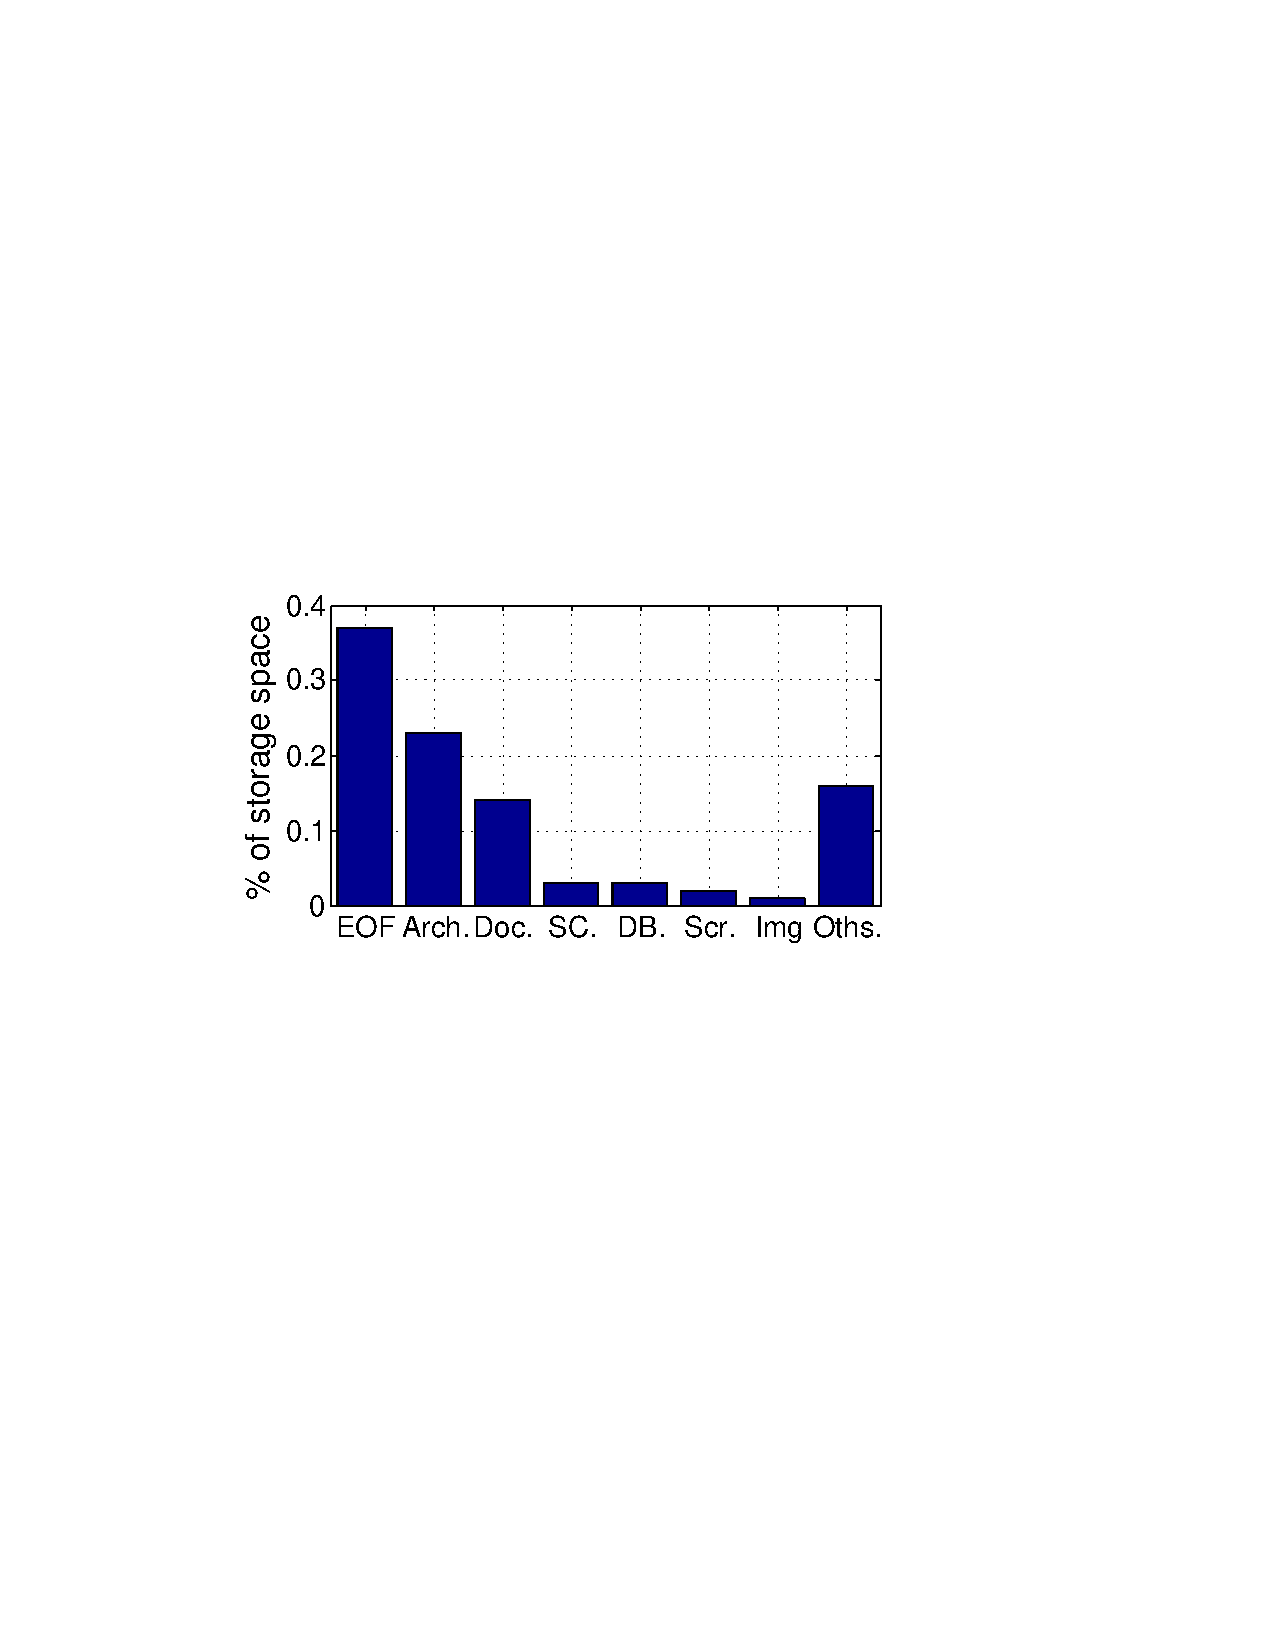
\includegraphics [width=0.225\textwidth]{graphs/type-total-size}
	}
	\caption{Common used file types}
	\label{fig:type-total}
\end{figure}

Figure~\ref{fig:type-total} shows the 8 type groups in terms of file count and capacity.
13\%, 11\%, and 9\% of files are source code, EOF, and scripts. 
EOF occupy the most of capacity (37\%). 
We can infer that developers mostly use Docker to develop, build, and run applications. This finding align with that images package more source code and executables.

We also see that Docker developers conduct many other activities in addition to coding. 
For example, 44\% of files are documents that contains Microsoft office files, LaTex files, etc., which means that developers also do editing or other productivity and 4\% of files are image files that contains Photoshop images, video game images, etc, meaning that developers also do entertainment or entertainment related development.

xxx~\cite{xxxx} shows that there is relation between file type and file size. 
To find how file type relate to file size, we calculated the average file size by file type group as shown in
Figure~\ref{fig:type-total-avg-size}. We see that Database files are much bigger (978.8 KB) than the files within other type groups. The average size of EOF and Archival files are around 100 KB. 
\textit{This finding is especially important for designer to optimize image size or mitigate registry storage overhead based on different file type}

%\begin{figure}
%	\centering
%	\subfigure[File count (in \%) by file type group.]{\label{fig:type-total-avg-size}
%		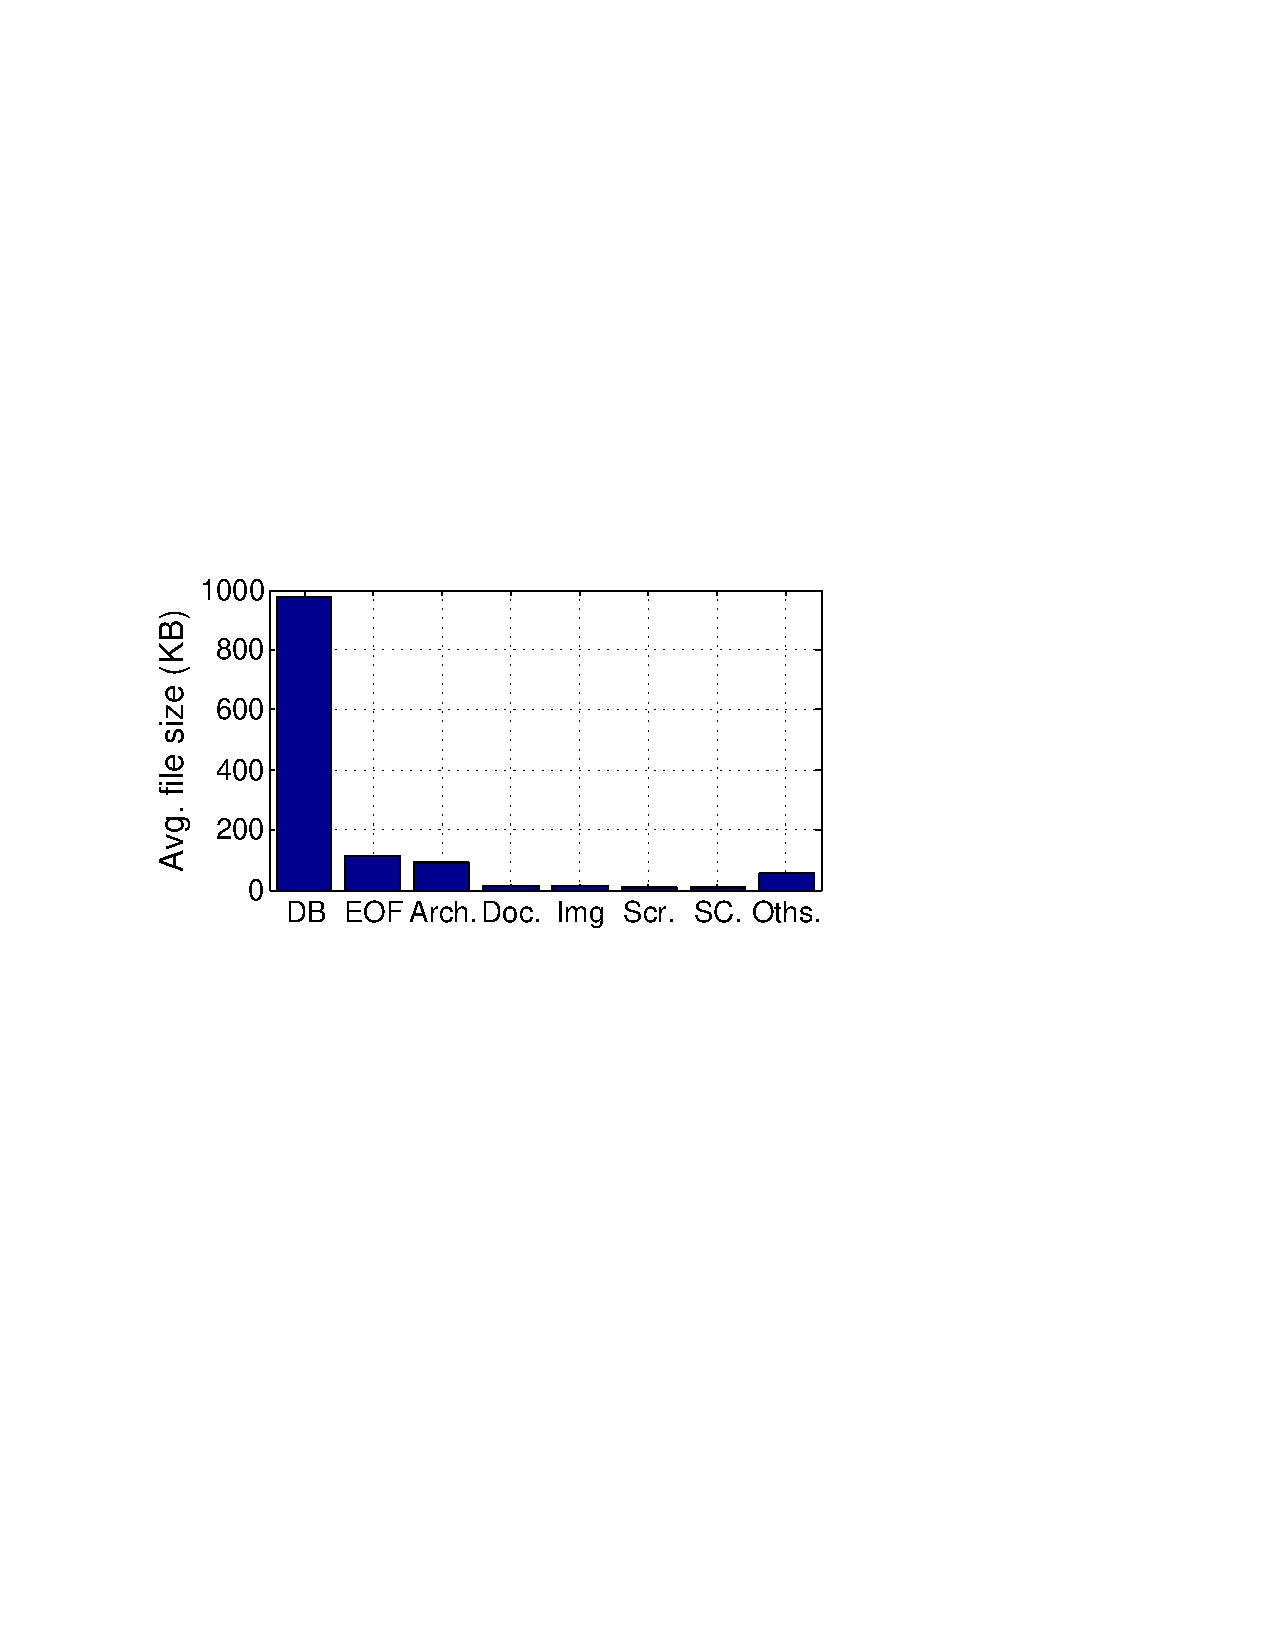
\includegraphics [width=0.225\textwidth]{graphs/type-total-avg-size}
%	}
%	\subfigure[Capacity (in \%) by file type group.]{\label{fig:type-total-size}
%		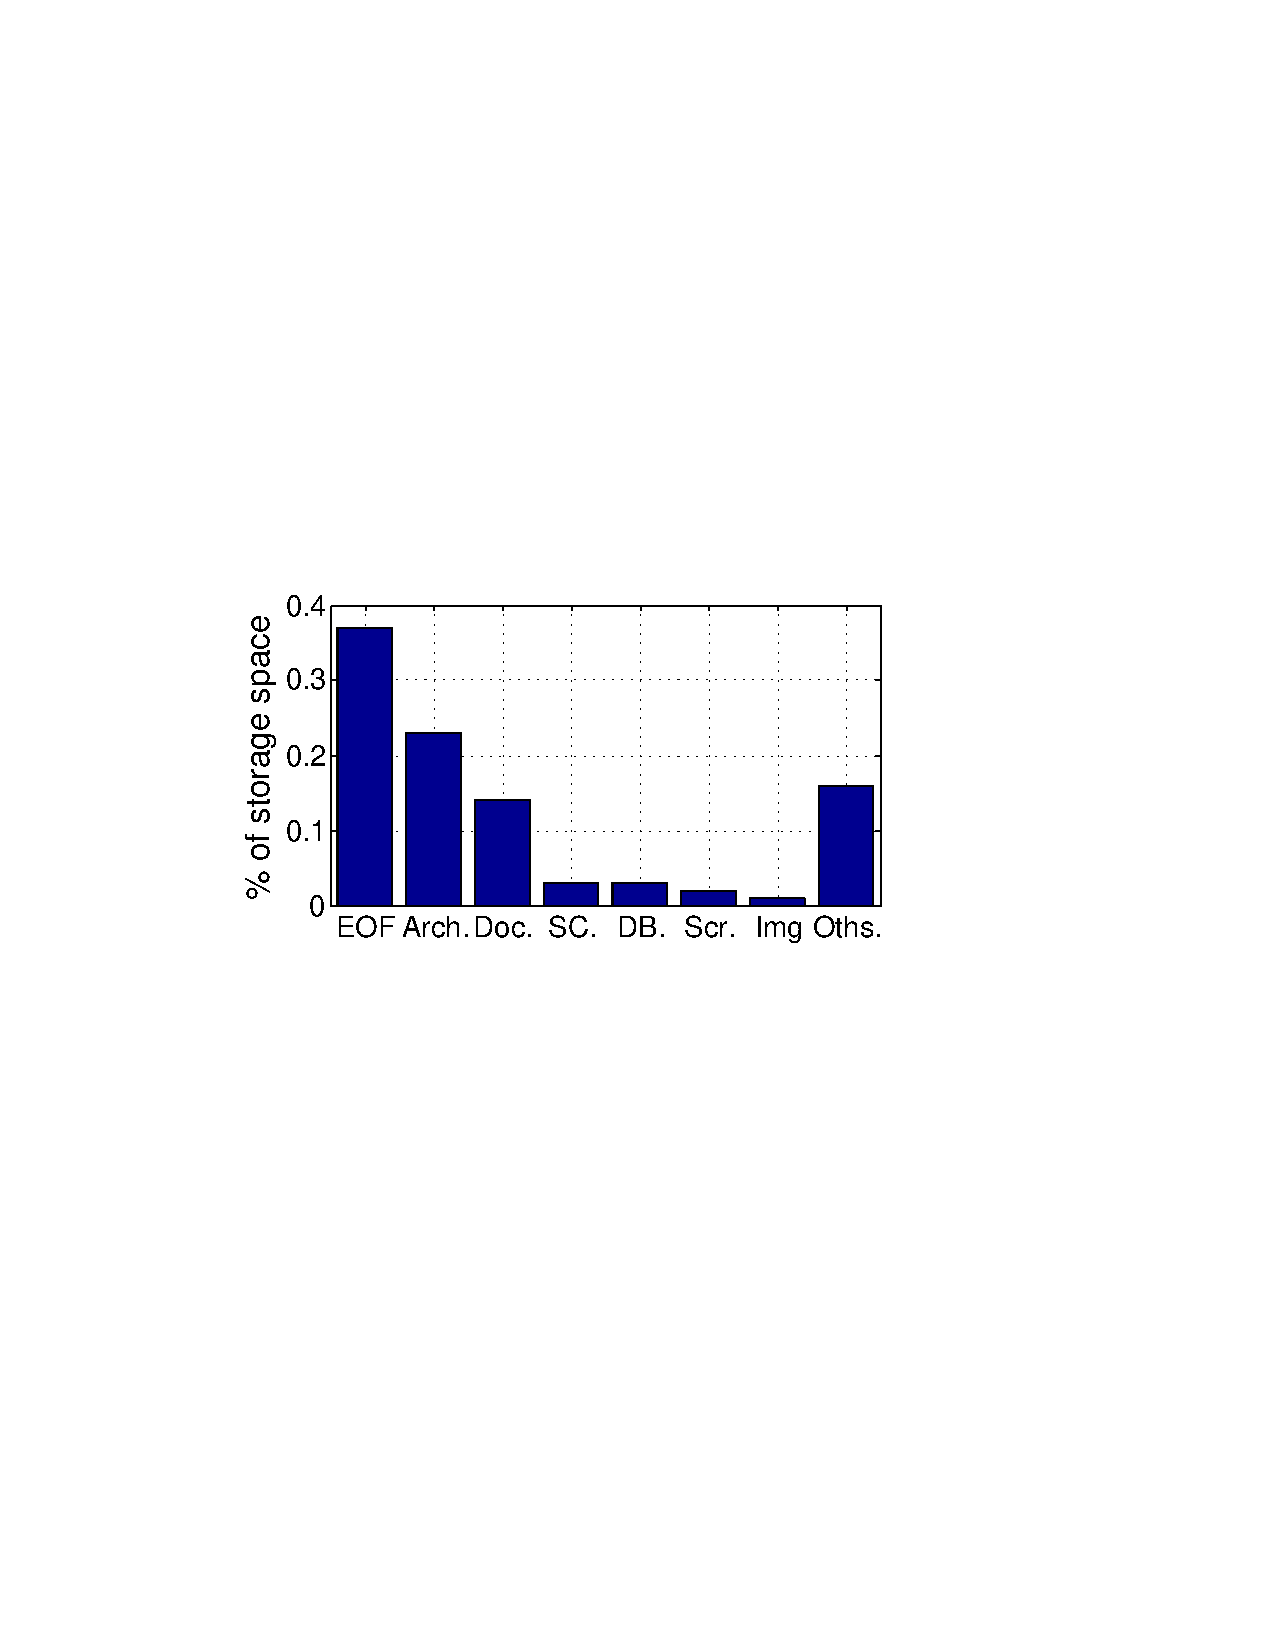
\includegraphics [width=0.225\textwidth]{graphs/type-total-size}
%	}
%	\caption{Common used file types}
%	\label{fig:type-total-size}
%\end{figure}

\begin{figure}[!t]
	\centering
	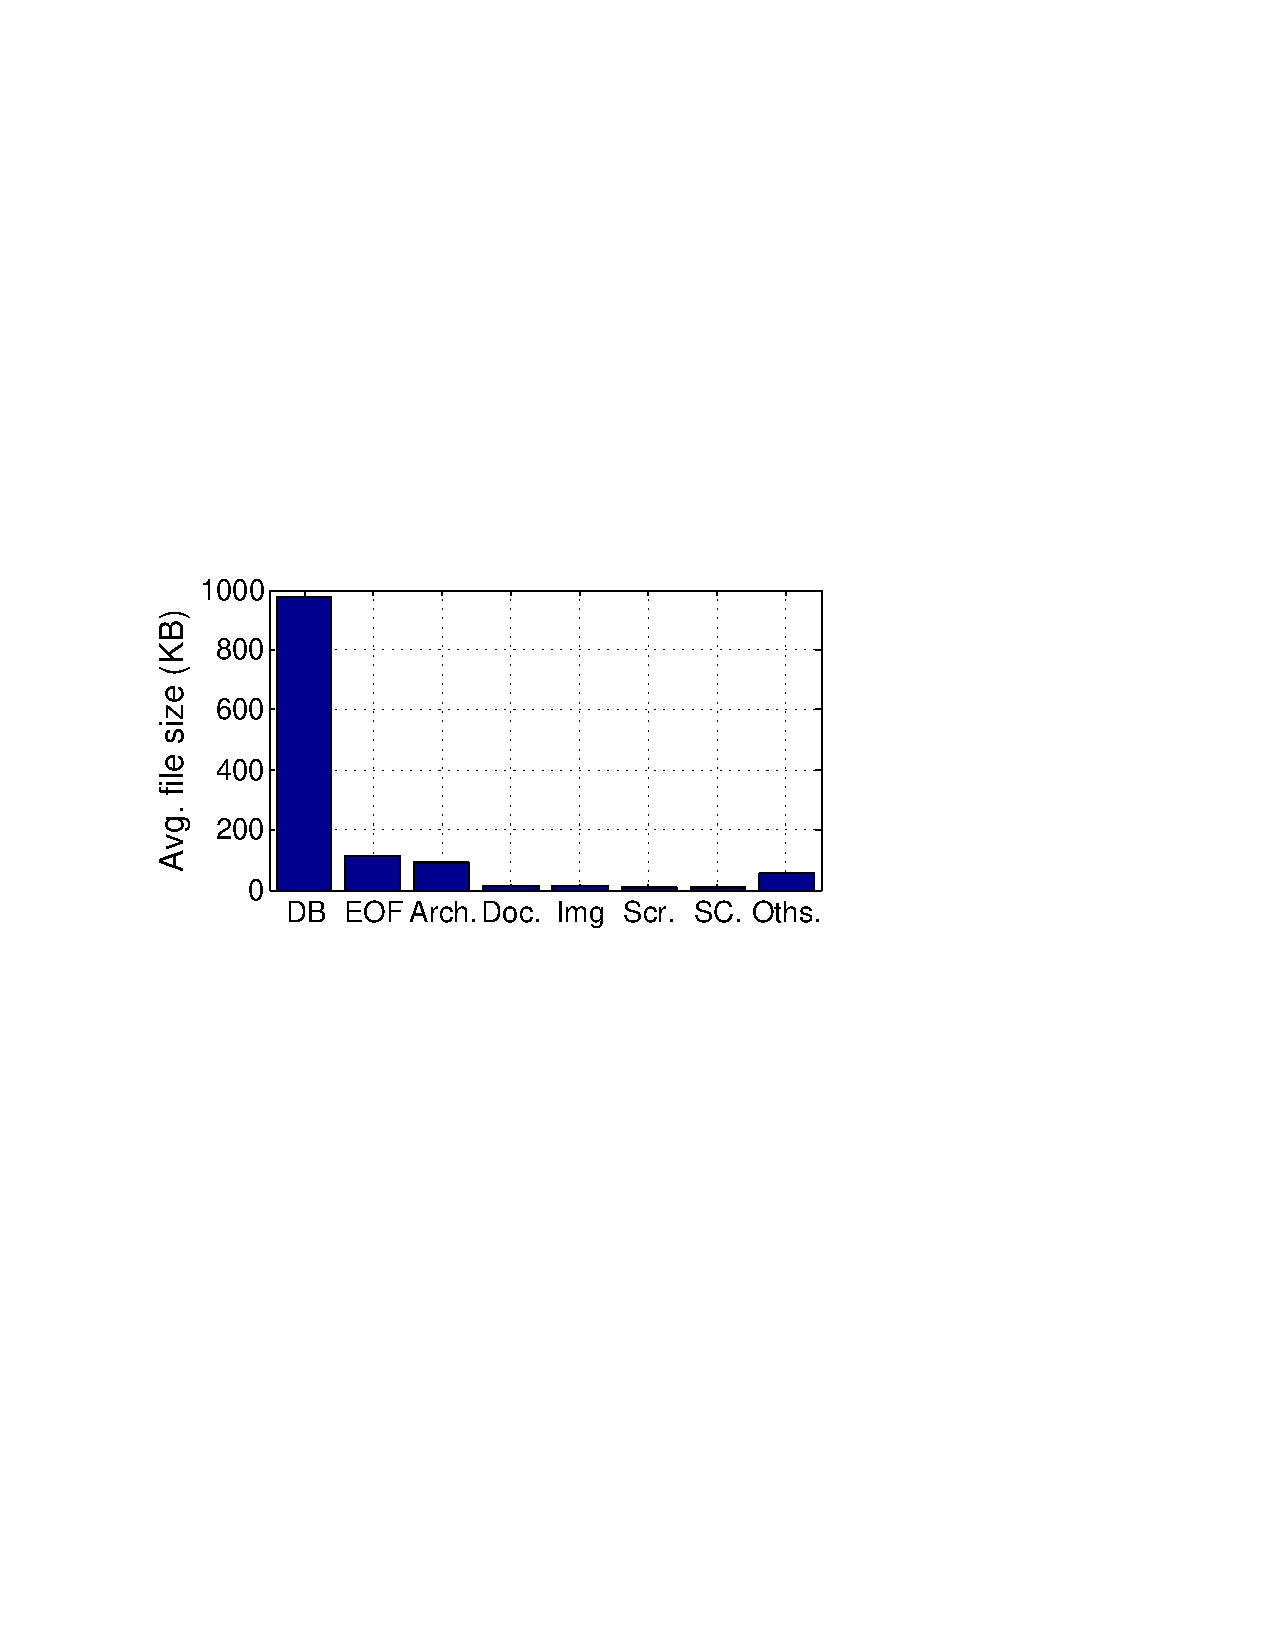
\includegraphics [width=0.225\textwidth]{graphs/type-total-avg-size}
	\caption{Average file size by file type group.}
	\label{fig:type-total-avg-size}
\end{figure}

% or further classify the redundant files based on involved by each file type. 
%We selected the file types which take largest storage space.

\paragraph{Executable, object code, and libraries (EOL)}
Based on the second-and third-classification, we further investigate the file size and file count by specific file types. We first start with EOF type group.
Figure~\ref{fig:type-eof} shows file type distribution in terms of file count and capacity for EOL type group. 
We see that majority of EOL files are ELF and intermediate complied files. ELF files contains ELF relocatable, shared object, and executables. Intermediate compiled files mainly contains Python Byte-compiled files, compiled java class, and terminfo compiled files. Although intermediate compiled files take up to 64\% of EOL files, 30\% of EOL files occupy 84\% of storage space consumed by EOL group. 
This is because average ELF file size is 312.7 KB while average intermediate compiled file size is 9 KB.

\textit{We conclude that among all file types, ELF files occupy most capacity. There are large amount of intermediate compiled files but they take very less storage space.}

\begin{figure}
	\centering
	\subfigure[File count (in \%) by file type.]{\label{fig:type-eof-cnt}
		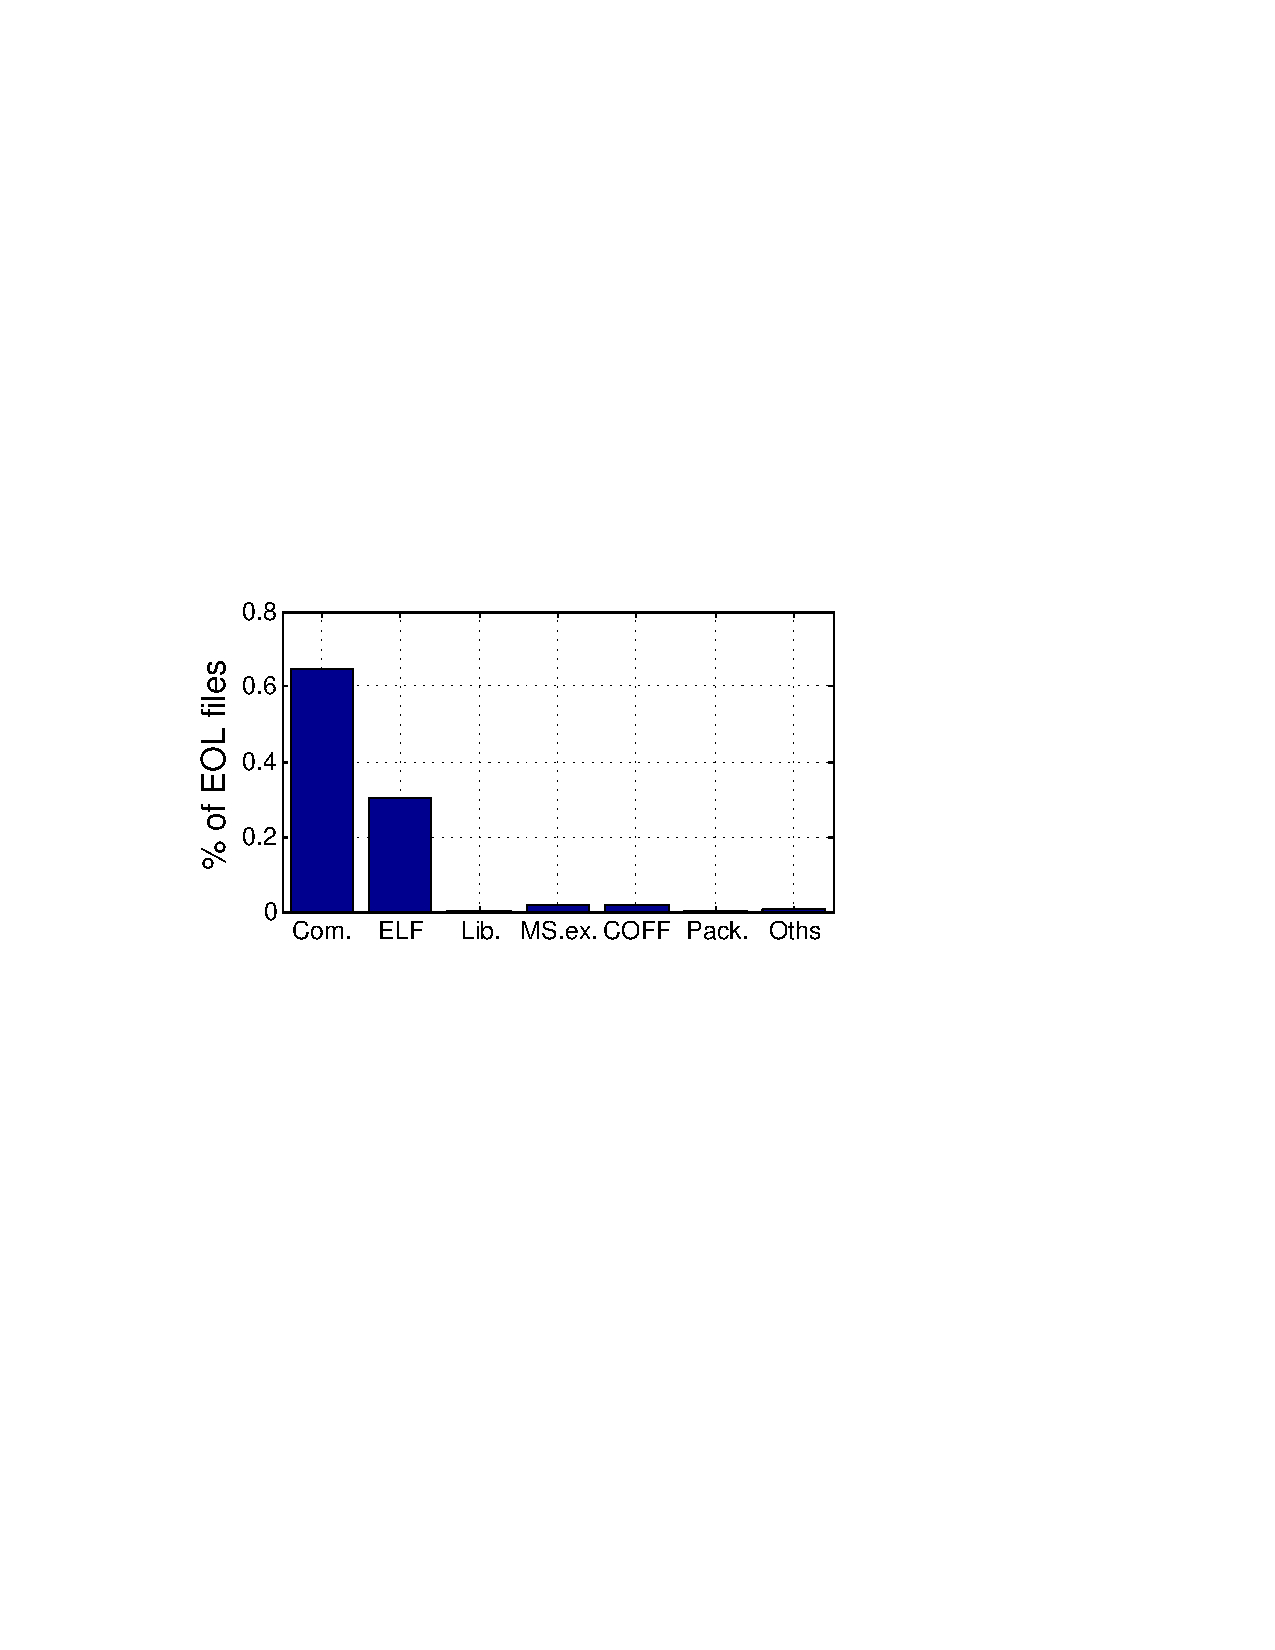
\includegraphics [width=0.225\textwidth]{graphs/type-eof-cnt}
	}
	\subfigure[Capacity (in \%) by file type.]{\label{fig:type-eof-size}
		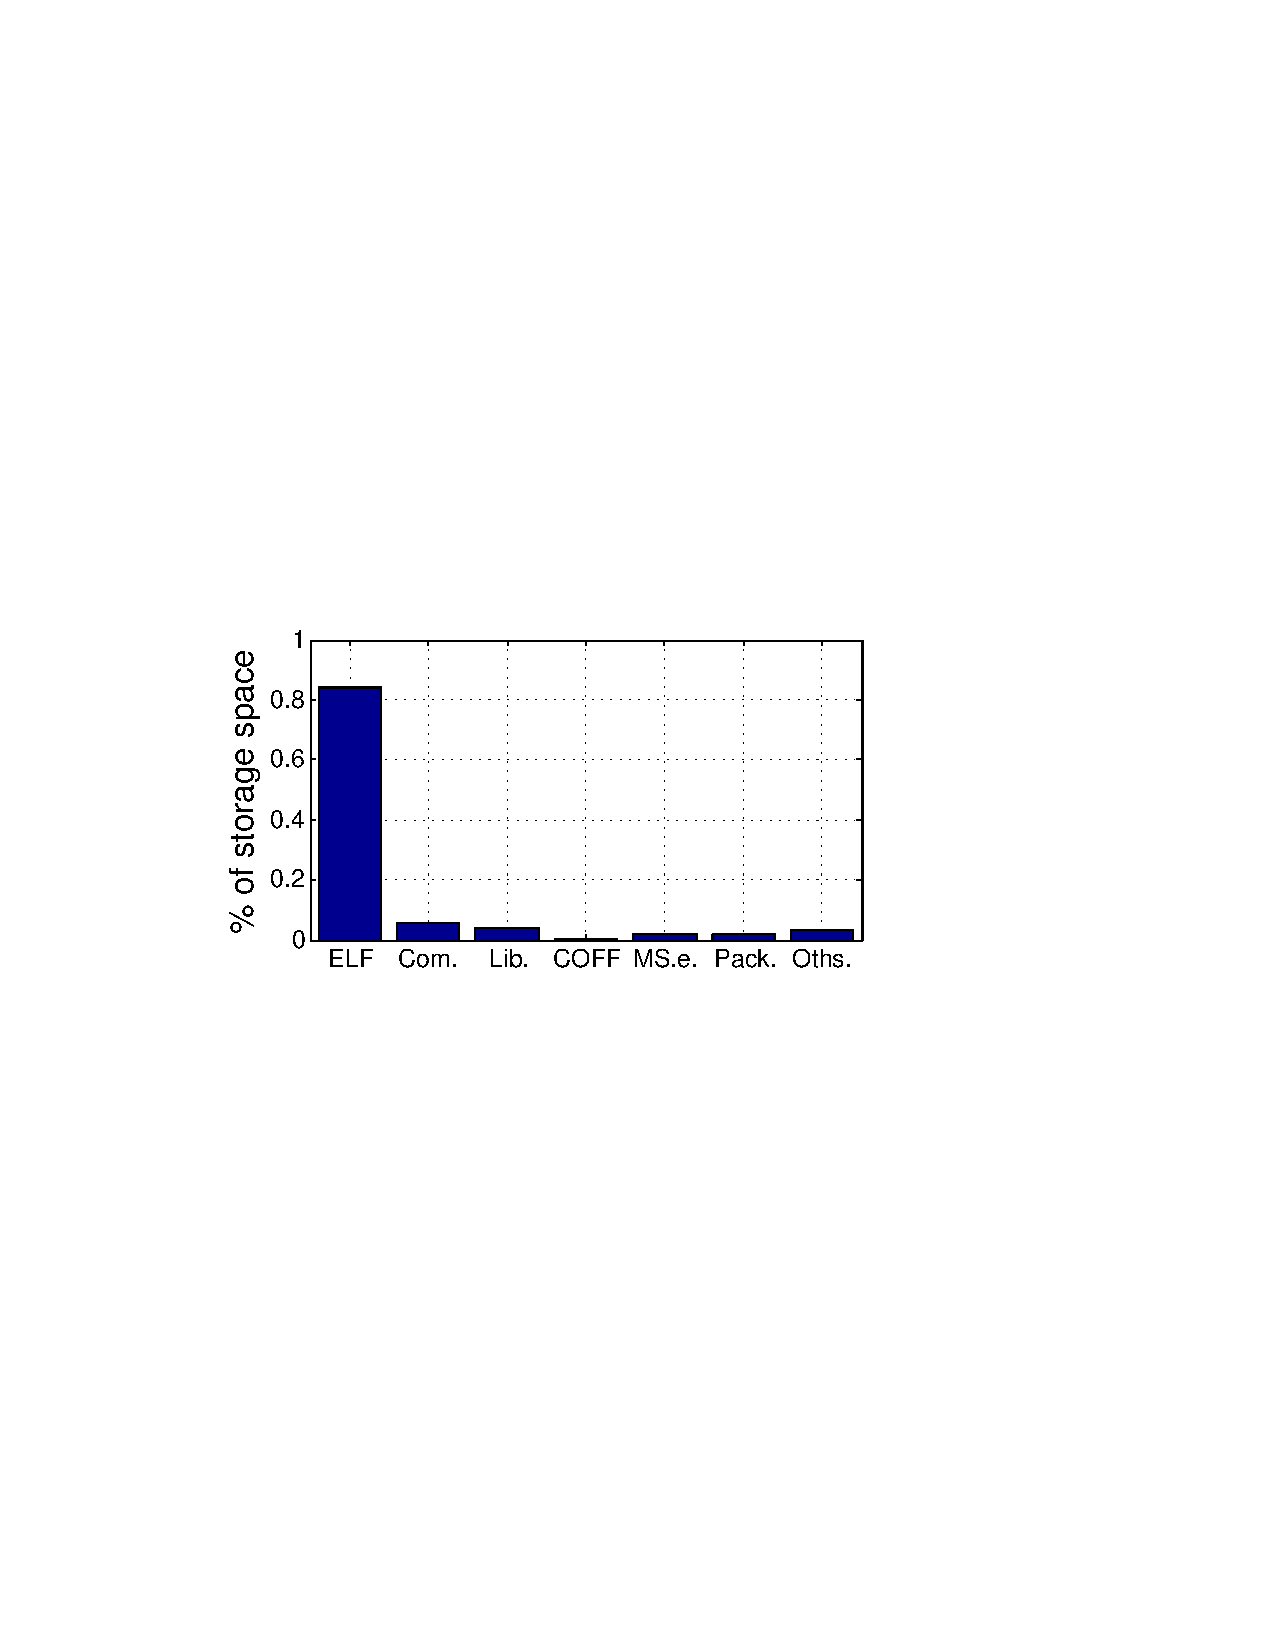
\includegraphics [width=0.225\textwidth]{graphs/type-eof-size}
	}
	\caption{EOL files}
	\label{fig:type-eof}
\end{figure}

We also find 0.2\% of EOL files are libraries, which contains 
There are Microsoft executables (2\%) in the dataset, meaning that developers also use other operating systems in addition to Linux.   

\paragraph{Source code (SC.)}


\paragraph{scripts (Scr.)}

\paragraph{Documents (Doc.)}

\paragraph{Archival (Arch.)}

\paragraph{Images (Img.)}

\paragraph{Databases (DB.)}

%, , archival, images, databases, and others
%\paragraph{Overall file size}

%\begin{figure}
%	\centering
%	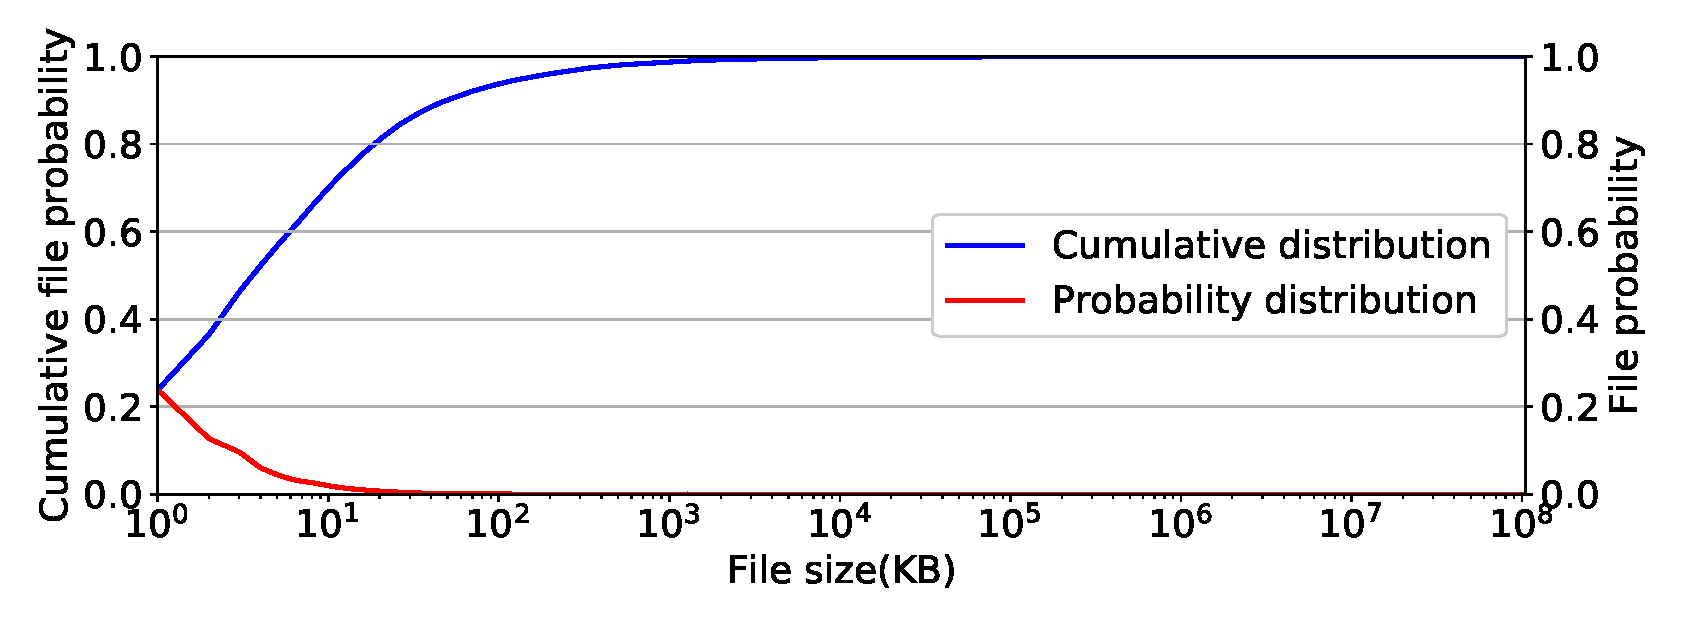
\includegraphics[width=0.5\textwidth]{graphs/File_size-KB.eps}
%	\caption{File size distribution.
%	}
%	\label{fig:file-size}
%\end{figure}
%
%Figure~\ref{fig:file-size} shows cumulative and probability distribution of file size.
%%of unique dataset after we remove the redundant files.
%\textit{Most files are smaller files.} For example, 91\% files are equal or less than 100 KB. 
%Around 22\% of files are less than 1 KB. 
%\textit{This is consistent with our finding that the layer size and image size are small both in compressed and uncompressed format.}  


%\subsection{File repeat count}
%\subsection{File size}


%As shown in Table~\ref{fig_image_growth}, the number of repositories increased
%linearly during our observation period from May 30th to September 20th,
%2017. Note that the graph shows a gap of 15 days due to Docker Hub changing the way it
%indexes repositories. The total number of repositories
%grew from 633,915 to 687,292, resulting in an average creation rate of 1,241
%repositories per day.
%This rapid growth of repositories suggests that storage optimizations will
%be crucial for registries in the neear future.
%Notice also,
%that each repository contains multiple tagged images and, therefore, we 
%significantly underestimatet the size of Docker Hub's content.